\documentclass[12pt]{article}
\usepackage{listings}
\usepackage{fontspec}
\usepackage{indentfirst}
\usepackage{graphicx}
\def\changemargin#1#2{\list{}{\rightmargin#2\leftmargin#1}\item[]}
\let\endchangemargin=\endlist 
\usepackage[margin=1 in]{geometry}
\usepackage{pdfpages}
\linespread{1} 


  %-----------------------------------------------------------------------
  \setromanfont{Times New Roman}
  %-----------------------------------------------------------------------

\begin{document}
\title{Report:  Managing Operations \\ A Case Study in Operations Research}

\author
{Zhengze Yu\thanks{yuzhengze@ict.ac.cn\quad 201928013229043 \quad The School of Computer Science and Technology },
\& Xinpeng Jin\thanks{jinxinpeng@mails.ucas.ac.cn\quad 201828015651001 \quad
College of Advanced Agricultural Science}
\\University of Chinese Academy of Sciences}
    \maketitle
        \begin{center}
            
\includegraphics[width=0.5\linewidth]{figure/logo.pdf}\\[4ex]
        \end{center}
    \setcounter{page}{1}
	\pagenumbering{gobble}
    %Add content for page two here (useful for two-sided printing)
    \thispagestyle{empty}
    \newpage
	\pagenumbering{arabic}
	
\section{Description of Problem}
Golf-Sport is a small-sized company that produces high-quality components for people who build their own golf clubs and prebuilt sets of clubs. There are five components:  steel shafts, graphite shafts, forged iron heads, metal wood heads, and metal wood heads with titanium inserts; these products are produced in three plants:  Chandler, Glendale, and Tucson. Each plant can produce any of the components, although each plant has a different set of individual constraints and unit costs. These constraints cover labor and packaging machine time (the machine is used for all components). Note that even though the components are identical in the three plants, different production processes are used, and therefore the products use different amounts of resources in different plants.
\par
Besides component sales, the company takes the components and manufactures sets of golf clubs. Each set requires 13 shafts, 10 iron heads, and 3 wood heads. All of the shafts in a set must be the same type (steel or graphite), and all of the wood heads must be the same type (metal or metal with inserts). Each plant has unique assembly times.  Furthermore, each plant of Golf-Sport has a retail outlet to sell components and sets, and the specific plant is the only supplier for its retail outlet. The minimum and maximum amounts of demand for each location are unique.
\par
This planning problem is for two months. The material, production, and assembly costs increase by 12\% for the second month, and production times are stationary. Inventory costs are based on end-of-period inventory for each product set and cost out at 8\% of the cost values of material, production and assembly. Additionally, each product generates different revenue depending on where it is made. Initially, there is no inventory.
\par
The corporation controls the capital available or expenses; the cash requirements for each product are given. There is a total of \$20,000 available for advertising for the entire system during each month, and any money not spent in a month is not available the next month. The corporation also controls graphite. Each shaft requires 4 ounces of graphite; a total of 1,000 pounds is available for each of the two months. 
\par

Your job is to determine a recommendation for the company. A recommendation must include a plan for production and sales. In addition, you should also address the following sensitivity-analysis issues in your recommendation:

\begin{itemize}
	\item If you could get more graphite or advertising cash, how much would you like, how would you use it, and what would you be willing to pay?
	\item At what site(s) would you like to add extra packing machine hours, assembly hours, and/or extra labor hours? How much would you be willing to pay per hour and how many extra hours would you like?
	\item Marketing is trying to get Golf-Sport to consider an advertising program that promises a 50\% increase in their maximum demand. Can we handle this with the current system or do we need more resources? How much more is the production going to cost if we take on the additional demand?
\end{itemize}
\par

%Key Words: Linear programming, Production process, Inventory balanced constraints, Sensitivity-analysis.

The solution will presented as a linear programming form with a single objective function to be maximized the profit and constraints based on the production process ,inventory balanced mentioned in the description of the problem. The recommendation will addressed by sensitivity-analysis after solving the linear programming problem.

\newpage

\section{Formulation \& Model}

\subsection{Observation of Problem}
In this problem, the decision variables can be considered into the following parts: production factory and period.
\begin{itemize}

    \item PRODUCTION = $\{$
        Basic\,Components, Assembled\,Sets
    $\}$
    Where \\Basic\,Components include:
\begin{center}
\begin{tabular}{ c }
\hline
\textbf{Product} \\
\hline
 Steel Shafts \\
 Graphite Shafts \\
 Forged Iron Heads \\
 Metal Wood Heads \\
 Titanium Insert Wood Heads \\
\hline
\end{tabular}
\vspace{5mm}
\end{center}

\noindent
And the Basic Components can be further descried as:\\
Basic Components = $\{$
        shafts,iron-heads, wood-heads
    $\}$
    
\noindent
    Assembled\,Sets include:

\begin{center}
\begin{tabular}{ c }
\hline
\textbf{Product} \\
\hline
 Steel Shafts \\
 Set, Steel Shafts, Metal Heads \\
 Set, Steel Shafts, Insert Heads \\
 Set, Graphite Shafts, Metal Heads \\
 Set, Graphite Shafts, Insert Heads \\
\hline
\end{tabular}
\vspace{5mm}
\end{center}


    % \item MANUFACTURE: M \\ determining the manufacturing process. 
    % \item SALE: X \\  determining  manufacturing and production process
    % \item INVENTORY: I \\ in terms of production process and inventory 
    % \item ADVERTISEMENT:A \\in terms of investment in advertising.
    \item FACTORY = $\{$
        Chandler,Glendale,Tuson
    $\}$
    \item PERIOD = $\{$
        0,1,2
    $\}$
    
    There are three specific aspects that the production should be took into account:
    \begin{itemize}
        \item Manufacture: $M = m_{ijt}$
        \item Sale :$S = x_{ijt}$
        \item Inventory: $I = v_{ijt}$
    \end{itemize}
Where

$i \in PRODUCTION$,
$j \in FACTORY$,
$t \in PERIOD$

\end{itemize}
\par

Besides decision variables, there are two types of constraints in this problem: local and global. Local constraints confined within identical production manufactured at certain factory in particular period(e.g. the minimum and maximum amounts of demand for each plant-product pair) while global constraints sets the whole limitation in at least one of the three dimensions: production, factory and period(e.g. graphite and advertisement control).
\par

\subsection{Variables}

Based on the observation, we can formulate the variables in the model.

\begin{center}
\begin{tabular}{ c  c  c}
\hline
\textbf{Variable} & \textbf{Description} & \textbf{Type}\\
\hline
\textit{$m_{ijt}$} & Product \textit{i} manufactured in plant \textit{j} at month \textit{t} & number\\
\textit{$x_{ijt}$} & Product \textit{i} sold in plant \textit{j} at month \textit{t} & number\\
\textit{$v_{ijt}$} & Inventory \textit{i} remained in plant \textit{j} at month \textit{t} & number\\
\textit{$M_t$} & Manufacture Matrix at month\textit{t} & matrix\\
\textit{$B_t$} & Basic components manufacture Matrix at month\textit{t} & matrix\\
\textit{$S_t$} & Assemble components manufacture Matrix at month\textit{t} & matrix\\
\textit{$X_t$} & Sale Matrix at month\textit{t} & matrix\\
\textit{$I_t$} & Inventory Matrix at month\textit{t} & matrix\\
\textit{$Basic$} & Basic Components = $\{$
        $s,g,f,m,t$
    $\}$ 
    &enumerate set\\
\textit{$Assemble$} & Assembled Sets = $\{$
        $ssm,ssi,sgm,sgi$
    $\}$ 
    &enumerate set\\
\textit{shafts} & shafts = $\{$
        $s,g$
    $\}$ 
    &enumerate set\\
\textit{iron-heads} & iron-head = $\{$
        $f$
    $\}$ 
    &enumerate set\\
\textit{wood-heads} & wood-head = $\{$
        $m,t$
    $\}$ 
    &enumerate set\\
\textit{factory} & factory = $\{
        $Chandler,Glendale,Tuson
    $\}$ 
    &enumerate set\\
\hline
\end{tabular}
\vspace{5mm}
\end{center}
Where
$i\in
    \left\{
        s,g,f,m,t,ssm,ssi,sgm,sgi
    \right\}$
\noindent
$j\in
    \left\{
        Chandler,Glendale,Tuson
    \right\}$
$t=0,1,2$

\noindent

\subsection{Objective Function}

The objective of this model is to maximize profit, represented as the difference between sales revenue and cost.  For the purposes of this function let \textit{R, H, C} and \textit{A} represent revenue, product cost, and inventory cost, and advertisement cost respectively.  The function can be expressed as:
$$\max Z = Revenue-Inventory \quad cost-Production \quad cost-Advertisement$$
\begin{equation}
=
% RˆTX_t
\sum\limits_{t=1}^2{\mathrm {tr}(R ^ \mathrm{ T }X_t)}
- \sum\limits_{t=1}^2 {\mathrm {tr}(H_t ^ \mathrm{ T }I_t)} 
- \sum\limits_{t=1}^2 {\mathrm {tr}(C_t ^ \mathrm{ T }M_t)}
- \sum\limits_{t=1}^2 {\mathrm {tr}(A ^ \mathrm{ T }B_t)}
\end{equation}



(Note: $\mathrm {tr}(M)$ is the trace of a matrix M)

The total revenue from all products produced and sold, minus the cost of manufacture, inventory and advertising is represented in this function. 

\noindent
Where: R is the matrix indicate revenue generated by each product.
\begin{center}
$\mathbf{R} =  
\left[
\begin{array}{l c r}
10 &10 & 12  \\
25 &25 & 30  \\
8  &8  & 10  \\
18 &18 & 22  \\
40 &40 & 45  \\
290&290&  310  \\
380&380&  420  \\
560&560&  640  \\
650&650&  720  
\end{array}
\right]
$
\end{center}
\noindent
C is the matrix indicate costs generated by manufacturing:
$C= \left[C_1,C_1\times1.12\right]$

\begin{center}
$\mathbf{C_1} = 
\left[
\begin{array}{l c r}
6  & 5 & 7  \\
19 & 18& 20 \\
4  & 5 & 5  \\
10 & 11& 12 \\
26 & 24& 27 \\
294 &291 &325 \\
362 &363 &409 \\
492 &502 &580 \\
580 &604 &684 
% 178  &175  & 180  \\
% 228  &220  & 240  \\
% 350  &360  & 370  \\
% 420  &435  & 450  
\end{array}
\right]
$
\end{center}

\begin{center}
$\mathbf{C_2} =  
\left[
\begin{array}{l c r}
6.72 &5.60 &7.84 \\
21.28 &20.16 &22.40 \\
4.48 &5.60 &5.60 \\
11.20 &12.32 &13.44 \\
29.12 &26.88 &30.24 \\
297.6 &294.24 &325.36 \\
365.84 &366.96 &411.16 \\
495.96 &507.16 &582.88 \\
586.60 &613.48 &691.08
% 199.36 &196.00 &201.60 \\
% 255.36 &246.40 &268.80 \\
% 392.00 &403.20 &414.40 \\
% 470.40 &487.20 &504.00 \\

\end{array}
\right]
$
\end{center}
\noindent
H is the matrix indicate costs generated by hiring warehouse for inventory.
\\$H_t= C_t\times0.08$
\begin{center}
$\mathbf{H_1} =  
\left[
\begin{array}{l c r}
0.48 &0.40 &0.56 \\
1.52 &1.44 &1.60 \\
0.32 &0.40 &0.40 \\
0.80 &0.88 &0.96 \\
2.08 &1.92 &2.16 \\
2.40 &2.16 &0.24 \\
2.56 &2.64 &1.44 \\
2.64 &3.44 &1.92 \\
4.40 &6.32 &4.72 
\end{array}
\right]
$
\end{center}

\begin{center}
$\mathbf{H_2} =  
\left[
\begin{array}{l c r}
0.5376 &0.4480 &0.6272 \\
1.7024 &1.6128 &1.7920 \\
0.3584 &0.4480 &0.4480 \\
0.8960 &0.9856 &1.0752 \\
2.3296 &2.1504 &2.4192 \\
2.6880 &2.4192 &0.2688 \\
2.8672 &2.9568 &1.6128 \\
2.9568 &3.8528 &2.1504 \\
4.9280 &7.0784 &5.2864 
\end{array}
\right]
$
\end{center}

\noindent
A is the matrix indicate investment in advertisements.
\begin{center}
$\mathbf{A} = 
\left[
\begin{array}{l c r}
1.0 & 1.1 & 1.3 \\
1.5 & 1.1 & 1.3 \\
1.1 & 1.1 & 1.3 \\
1.5 & 1.2 & 1.3 \\
1.9 & 1.9 & 1.9 
% 0.0 & 0.0 & 0.0 \\
% 0.0 & 0.0 & 0.0 \\
% 0.0 & 0.0 & 0.0 \\
% 0.0 & 0.0 & 0.0
\end{array}
\right]
$
\end{center}

\noindent 

\subsection{Constraints}
\subsubsection{Local constraints}
\noindent
\textbf{Labor(workforce):}
\begin{equation}
diag(W^\mathrm{T}B)\leq W_c
\end{equation}

\noindent
where:\\
\begin{center}
$\mathbf{W} = 
\left[
\begin{array}{l c r}
1.0 & 3.5 & 3.0 \\
1.5 & 3.5 & 3.5 \\
1.5 & 4.5 & 4.0 \\
3.0 & 4.5 & 4.5 \\
4.0 & 5.0 & 5.5
\end{array}
\right]
$
\end{center}

\begin{center}
$\mathbf{W_c} = 
\left[
12,000\quad  15,000\quad  22,000
\right]
$
\end{center}

\noindent
\textbf{Packing machine:}
\begin{equation}
diag(P^\mathrm{T}B)\leq P_c
\end{equation}
Where:
\begin{center}
$\mathbf{P} = 
\left[
\begin{array}{l c r}
4.0 & 7.0 & 7.5 \\
4.0 & 7.0 & 7.5 \\
5.0 & 8.0 & 8.5 \\
6.0 & 9.0 & 9.5 \\
6.0 & 7.0 & 8.0
\end{array}
\right]
$
\end{center}

\begin{center}
$\mathbf{P_c} = 
\left[
20,000\quad  40,000\quad  35,000
\right]
$
\end{center}
\noindent
\textbf{Assembly time:}
\begin{equation}
T^\mathrm{T}
\sum\limits_{j\in factory} {S_j}
\leq T_c
\end{equation}
Where:
\begin{center}
$\mathbf{T} = 
\left[
65\quad  60\quad  65
\right]
$
\end{center}

\begin{center}
$\mathbf{T_c} = 
\left[
5,500\quad  5,000\quad  6,000
\right]
$
\end{center}
Demand:
\begin{equation}
L\leq M \leq U
\end{equation}
Where:
\begin{center}
$\mathbf{L} = 
\left[
\begin{array}{l c r}
0   & 0   & 0   \\
100 & 100 & 50  \\
200 & 200 & 100 \\
30  & 30  & 15  \\
100 & 100 & 100 \\
0   & 0   & 0   \\
0   & 0   & 0   \\
0   & 0   & 0   \\
0   & 0   & 0 
\end{array}
\right]
$
\end{center}

\begin{center}
$\mathbf{U} = 
\left[
\begin{array}{l c r}
2000 & 2000& 2000 \\
2000 & 2000& 2000 \\
2000 & 2000& 2000 \\
2000 & 2000& 2000 \\
2000 & 2000& 2000 \\
200  &200  & 200  \\
100  &100  & 100  \\
300  &300  & 300  \\
400  &400  & 400  
\end{array}
\right]
$
\end{center}
\noindent
\textbf{Production process and inventory constraints:}

To interpret "Each set requires 13 shafts, 10 iron heads, and 3 wood heads. All of the shafts in a set must be the same type (steel or graphite), and all of the wood heads must be the same type (metal or metal with inserts)." in a mathematical way, we have:\\
\begin{center}
    $13sht+10iron+3wood=set$\\
($sht\in shafts,iron\in iron-heads,wood\in wood-heads,set\in Assemble$)
\end{center}
i.e.
\begin{equation}
    F_1M_t+F_2S_t+F_3I_{t-1}+F_4I_t = 0
\end{equation}


\noindent
To be specific, for every $j\in \left\{Chandler,Glendale,Tuson\right\} t=1,2$ 

$$
13m_{ssm,j,t}+13m_{ssi,j,t}+x_{s,j,t}+v_{s,j,t}=m_{s,j,t}+v_{s,j,t-1}
$$

$$
13m_{sgm,j,t}+13m_{sgi,j,t}+x_{g,j,t}+v_{g,j,t}=m_{g,j,t}+v_{g,j,t-1}
$$

$$
10\sum\limits_{i\in Assembly} {m_{i,j,t}} + x_{f,j,t} + v_{f,j,t} = m_{f,j,t}+v_{f,j,t-1}
$$

$$
3m_{sgm,j,t}+3m_{ssi,j,t}+x_{m,j,t}+v_{m,j,t}=m_{m,j,t}+v_{m,j,t-1}
$$

$$
3m_{ssm,j,t}+3m_{ssi,j,t}+x_{t,j,t}+v_{t,j,t}=m_{t,j,t}+v_{t,j,t-1}
$$

\noindent
For every $i\in \left\{ssm,ssi,sgm,sgi\right\}$
$j\in \left\{Chandler,Glendale,Tuson\right\}
t=1,2$ 
$$
m_{i,j,t}+x_{i,j,t}-v_{i,j,t-1}+v_{i,j,t}=m_{i,j,t}
$$

\noindent
\subsubsection{Global constraints }
\noindent
\textbf{Advertising constraints:}
\begin{equation}
\mathrm {tr}(A ^ \mathrm{ T }B_t)\leq A_c
\end{equation}
$$A_c = \left[20,000\right]$$

\noindent
\textbf{Graphit constraints:}
\begin{equation}
\sum \limits_{j\in factory}{m_{g,j,t}}\leq G_c
\end{equation}
$$G_c = \left[4,000\right]$$





\section{Implementation \& Recommendation}

\subsection{Implementation \& Solution}
In order to encoding subscript $i,j$ in a more effective way, we encode subscript $i,j$ based on one-hot encoding, i.e. for index $i$:
$$
        s \to 1,
        g \to 2,
        f \to 3,
        m \to 4,
        t \to 5,
        ssm \to 6,
        ssi \to 7,
        sgm \to 8,
        sgi \to 9,
$$
for index $j$:
$$
        Chandler \to 1,
        Glendale \to 2,
        Tuson \to 3,
$$

For example, product \textit{Steel Shafts} manufactured at Tuson in the second month is expressed as: $m_{1,3,2}$.With these tricks mentioned above, Problem was successfully coded in Lingo, yielding a maximized profit of \$221659.9 for Golf-Sport as a company in the two month period.\par

$$ \max Z = 221659.9$$

\subsection{Plan for Production and Sales}
The optimal decision variables indicate the plan for production and sales, which is showed in the following tables.\par

\noindent
\begin{center}
%begin{table}
\begin{tabular}{ l c c }
\hline
\multicolumn{3}{c}{Optimal Chandler manufacture} \\
\hline
\textbf{Item} & \textbf{Month 1} & \textbf{Month 2} \\
Steel Shafts & 0 & 0 \\
Graphite Shafts & 867.14 & 100 \\
Iron Heads & 200 & 200 \\
Metal Wood Heads & 588.57 & 1100 \\
Titanium Insert Wood Heads & 2000 & 2000 \\
Set, Steel, Metal Heads & 0 & 0 \\
Set, Steel, Titanium Heads & 0 & 0 \\
Set, Graphite, Metal Heads & 0 & 0 \\
Set, Graphite, Titanium Heads & 0 & 0 \\
\hline
\end{tabular}
%end{table} dont remove
\vspace{5mm}
\\
\end{center}

\noindent
\begin{center}
%begin{table}
\begin{tabular}{ l c c }
\hline
\multicolumn{3}{c}{Optimal Chandler Sales} \\
\hline
\textbf{Item} & \textbf{Month 1} & \textbf{Month 2} \\
Steel Shafts & 0 & 0 \\
Graphite Shafts & 867.14 & 100 \\
Iron Heads & 200 &200 \\
Metal Wood Heads & 588.57 & 1100 \\
Titanium Insert Wood Heads & 2000 & 2000 \\
Set, Steel, Metal Heads & 0 & 0 \\
Set, Steel, Titanium Heads & 0 & 0 \\
Set, Graphite, Metal Heads & 0 & 0 \\
Set, Graphite, Titanium Heads & 0 & 0 \\
\hline
\end{tabular}
%end{table} dont remove
\vspace{5mm}
\\
\end{center}

\noindent
\begin{center}
%begin{table}
\begin{tabular}{ l c c }
\hline
\multicolumn{3}{c}{Optimal Glendale manufacture} \\
\hline
\textbf{Item} & \textbf{Month 1} & \textbf{Month 2} \\
Steel Shafts & 0 & 0 \\
Graphite Shafts & 1132.86 & 1132.86 \\
Iron Heads & 200 & 200 \\
Metal Wood Heads & 30 & 30 \\
Titanium Insert Wood Heads & 2000 & 2000 \\
Set, Steel, Metal Heads & 0 & 0 \\
Set, Steel, Titanium Heads & 0 & 0 \\
Set, Graphite, Metal Heads & 0 & 0 \\
Set, Graphite, Titanium Heads & 0 & 0 \\
\hline
\end{tabular}
%end{table} dont remove
\vspace{5mm}
\\
\end{center}

\noindent
\begin{center}
%begin{table}
\begin{tabular}{ l c c }
\hline
\multicolumn{3}{c}{Optimal Glendale Sales} \\
\hline
\textbf{Item} & \textbf{Month 1} & \textbf{Month 2} \\
Steel Shafts & 0 & 0 \\
Graphite Shafts & 1132.86 & 1132.86 \\
Iron Heads & 200 & 200 \\
Metal Wood Heads & 30 & 30 \\
Titanium Insert Wood Heads & 2000 & 2000 \\
Set, Steel, Metal Heads & 0 & 0 \\
Set, Steel, Titanium Heads & 0 & 0 \\
Set, Graphite, Metal Heads & 0 & 0 \\
Set, Graphite, Titanium Heads & 0 & 0 \\
\hline
\end{tabular}
%end{table} dont remove
\vspace{5mm}
\\
\end{center}

\noindent
\begin{center}
%begin{table}
\begin{tabular}{ l c c }
\hline
\multicolumn{3}{c}{Optimal Tuson manufacture} \\
\hline
\textbf{Item} & \textbf{Month 1} & \textbf{Month 2} \\
Steel Shafts & 0 & 0 \\
Graphite Shafts & 2000 & 2000 \\
Iron Heads & 100 & 100 \\
Metal Wood Heads & 331.58 & 331.58 \\
Titanium Insert Wood Heads & 2000 & 2000 \\
Set, Steel, Metal Heads & 0 & 0 \\
Set, Steel, Titanium Heads & 0 & 0 \\
Set, Graphite, Metal Heads & 0 & 0 \\
Set, Graphite, Titanium Heads & 0 & 0 \\
\hline
\end{tabular}
%end{table} dont remove
\vspace{5mm}
\\
\end{center}

\noindent
\begin{center}
%begin{table}
\begin{tabular}{ l c c }
\hline
\multicolumn{3}{c}{Optimal Tuson Sales} \\
\hline
\textbf{Item} & \textbf{Month 1} & \textbf{Month 2} \\
Steel Shafts & 0 & 0 \\
Graphite Shafts & 2000 & 2000 \\
Iron Heads & 100 & 100 \\
Metal Wood Heads & 331.58 & 331.58 \\
Titanium Insert Wood Heads & 2000 & 2000 \\
Set, Steel, Metal Heads & 0 & 0 \\
Set, Steel, Titanium Heads & 0 & 0 \\
Set, Graphite, Metal Heads & 0 & 0 \\
Set, Graphite, Titanium Heads & 0 & 0 \\
\hline
\end{tabular}
%end{table} dont remove
\vspace{5mm}
\\
\end{center}

\subsection{Sensitive-analysis \& Recommendation}

After solving the linear programming problem, recommendations are made towards the issues proposed in the description of problem based on the solution report.

\begin{itemize}

	\item \textbf{issue:} If you could get more graphite or advertising cash, how much would you like, how would you use it, and what would you be willing to pay?
	
	\item \textbf{recommendation:}
	We selected several essential indexes from lingo lindo’s default solution and range reports dual price and allowable range to further analysis.
The shadow price and surplus of advertising and graphite is 0.67 and 0 respectively, suggesting investing 209.46 in graphite in the first month, yielding \$ 213,544.6 profit.\par
\begin{center}
\begin{tabular}{c c c c c c }
\hline
\multicolumn{6}{c}{range reports} \\
\ \textbf{month} &\textbf{Item} &\textbf{RHS} & \textbf{Allowable increase} & \textbf{Allowable decrease} &  \textbf{Dule price}\\
\hline
Month 1     &Graphite    &1000       &209.4643   &191.7857        &0.67\\
Month 2     &Graphite    &1000       &INF        &191.7857    &0\\
Month 1     &Advertising    &20,000     &INF    &1533.233        &0\\
Month 2     &Advertising    &20,000     &INF    &1916.855       &0\\
\hline
\end{tabular}
\end{center}


	
	\item \textbf{issue:} At what site(s) would you like to add extra packing machine hours, assembly hours, and/or extra labor hours? How much would you be willing to pay per hour and how many extra hours would you like?
	

	\item \textbf{recommendation:}
% 	延长人工作业时限对Chandler和Tucson获取更高收益无益,因此该两厂不必延长工时限制。只有Glendale对延长人工时限有响应,在第一个月增加单位时长能够获取1.64美元,第二个月1.069美元,总收益能分别增加4403和2870美元。延长机器打包时限能使Chandler和Tucson在第一个月分别额外获取1.083和0.916美元/小时,第二个月分别为0.883和0.764美元/小时,而对Glendale工厂是nonbinding的。最后我们发现延长装配时限对所有工厂都没有增加收益的作用,因此不建议延长装配时限。至于对延长时间所支付的价格,只要不大于其对应的影子价格即可。
		According to Righthand Side Ranges of labor and packaging constraints showed above, 
		adding extra labor time doesn't work for factory Chandler and Tucson whereas increasing profit for factory Glendale at \$1.64 in the first month and \$1.069 the second month per minute yielding profit \$4,403 and \$2,870, respectively.
		
		\par
		When it comes to extra packing and assembly time, report showed extra packing time increasing\$1.083 and\$0.916 in the first month for Chandler and Tucson respectively,\$0.883 and \$0.764 for the second. We notice that extra assembly time make no difference for any of three factory in any period.
		\par
		In conclusion, we suggest adding extra labor and packing time as long as it is not greater than its corresponding shadow price.
		\par
% 		I would(not) like to add extra packing machine hours, assembly hours, and/or extra labor hours. I'm willing to pay ***\$ per hour and *** extra hours no more than ***.
	
% 	IExtending the time limit for manual operations is not beneficial for Chandler and Tucson to obtain higher profit, so the two plants do not have to extend working hours. Only Glendale responded to the extension of the artificial time limit. In the first month, the unit time was increased by \$1.64, and the second month was \$1.069. The total revenue was increased by \$4,403 and \$2,870, respectively. Extending the machine packaging timeframe allowed Chandler and Tucson to receive an additional \$1.083 and \$0.916/hour in the first month, respectively, and \$0.883 and \$0.764/hour in the second month, respectively, and nonbinding for the Glendale plant. Finally, we found that extending the assembly time limit has no added benefit for all plants, so it is not recommended to extend the assembly time limit. As for the price paid for the extended time, as long as it is not greater than its corresponding shadow price.
	
\begin{center}
\begin{tabular}{c c c c c c }
\hline
\multicolumn{6}{c}{Labor} \\
\ \textbf{month} &\textbf{Factory} &\textbf{RHS} & \textbf{Allowable increase} & \textbf{Allowable decrease} &  \textbf{Dule price}\\
\hline
Month 1     &Chandler  &12,000    &INF   &633.57    &0\\
Month 1     &Glendale  &15,000    &2,685 &2,932.5   &1.64\\
Month 1     &Tucson    &22,000    &INF   &2,107.895 &0\\
Month 2     &Chandler  &12,000    &INF   &250       &0\\
Month 2     &Glendale  &15,000    &2,685 &3,615     &1.069\\
Month 2     &Tucson    &22,000    &INF   &2,107.9   &0\\
\hline
\end{tabular}
\end{center}

\begin{center}
\begin{tabular}{c c c c c c }
\hline
\multicolumn{6}{c}{Packing} \\
\ \textbf{month} &\textbf{Factory} &\textbf{RHS} & \textbf{Allowable increase} & \textbf{Allowable decrease} &  \textbf{Dule price}\\
\hline
Month 1     &Chandler  &20,000    &1,267.14   &3,351.43    &1.083\\
Month 1     &Glendale  &40,000    &INF      &16,200   &0\\
Month 1     &Tucson    &35,000    &4,450   &3,007.5 &0.916\\
Month 2     &Chandler  &20,000    &500      &6,420       &0.883\\
Month 2     &Glendale  &40,000    &INF       &16,200     &0\\
Month 2     &Tucson    &35,000    &4,450   &3,007.5   &0.764\\
\hline
\end{tabular}
\end{center}

\begin{center}
\begin{tabular}{c c c c c c }
\hline
\multicolumn{6}{c}{Assembly} \\
\ \textbf{month} &\textbf{Factory} &\textbf{RHS} & \textbf{Allowable increase} & \textbf{Allowable decrease} &  \textbf{Dule price}\\
\hline
Month 1     &Chandler  &5,500    &INF   &5,500    &0\\
Month 1     &Glendale  &5,000    &INF   &5,000   &0\\
Month 1     &Tucson    &6,000    &INF   &6,000 &0\\
Month 2     &Chandler  &5,500    &INF   &5,500       &0\\
Month 2     &Glendale  &5,000    &INF   &5,000     &0\\
Month 2     &Tucson    &6,000    &INF   &6,000  &0\\
\hline
\end{tabular}
\end{center}

	\item \textbf{issue:} Marketing is trying to get Golf-Sport to consider an advertising program that promises a 50\% increase in their maximum demand. Can we handle this with the current system or do we need more resources? How much more is the production going to cost if we take on the additional demand?
	
	\item \textbf{recommendation:}When we increase the maximum demand limit by 50\% in our model i.e.

\begin{center}
$\mathbf{U'} = 
\left[
\begin{array}{l c r}
3000 & 3000& 3000 \\
3000 & 3000& 3000 \\
3000 & 3000& 3000 \\
3000 & 3000& 3000 \\
3000 & 3000& 3000 \\
300  &300  & 300  \\
150  &150  & 150  \\
450  &450  & 450  \\
600  &600  & 600  
\end{array}
\right]
$
\end{center}

\begin{center}
\begin{tabular}{c c c c c c }
\hline
\multicolumn{6}{c}{Assembly} \\
\ \textbf{month} &\textbf{Factory} &\textbf{RHS} & \textbf{Allowable increase} & \textbf{Allowable decrease} &  \textbf{Dule price}\\
\hline
Month 1     &Chandler  &5,500    &INF   &5,500    &0\\
Month 1     &Glendale  &5,000    &INF   &5,000   &0\\
Month 1     &Tucson    &6,000    &INF   &6,000 &0\\
Month 2     &Chandler  &5,500    &INF   &5,500       &0\\
Month 2     &Glendale  &5,000    &INF   &5,000     &0\\
Month 2     &Tucson    &6,000    &INF   &6,000  &0\\
\hline
\end{tabular}
\end{center}

which exceeds the allowable change causing optimal value $Z'$ comes to \$241,175 suggesting that more resource is needed. We consider the production cost no more than \$27,770 in total.
% , the revised  
% 	optimal value $Z'$ comes to \$241,175, which is higher than the original  $Z = $ \$223,405, indicating that the profit remained in \$223,405 unless increase the limit of resources. \par
% 	By comparison, we found that the former rof's decreased cost multiplied non-negative basic value confined optimal value in \$223,405, but when maximum demand increases 50 percent i.e.
	
% 	, many basic value’s decreased cost come to zero,  no longer play a negative effect to the optimal value.
	%因此在不考虑改变售价的情况下,达到这一最大收益只能通过增加资源的供给来实现,反过来说,也即当前资源是不足以满足扩大50%的去求,不足以获取这一更高的Z值。通过比较二者结果报告可以发现在现状下存在更多的变量由于需求量的约束处于变量为正、Reduced cost 为负的状态,而当需求扩大后这种情况减少,收益潜力被释放。
% \begin{center}
% \begin{tabular}{ c c c c }
% \hline
% \multicolumn{4}{c}{Righthand Side Ranges:} \\
%  &\textbf{Current} & \textbf{Allowable} & \textbf{Allowable} \\
% \hline
% ROW      &RHS                 &Increase            &Decrease\\
% 1        &370.0000            &1.000000            &    0\\
% 2        &1.200000            &0.000000            &    0\\
% 3        &0.000000            &10.00000            &    0\\
% 4        &0.000000            &-1.000000           &    0\\
% \hline
% \end{tabular}
% \end{center}



	
\end{itemize}

\section{Contributions}
Yu
\begin{itemize}
	\item Modeling.
	\item Writing report.
\end{itemize}

Jin
\begin{itemize}
	\item Checking correctness of model. 
	\item Programming.
	\item Sensitivity Analysis.
\end{itemize}

\newpage
\section{Appendix}
\begin{changemargin}{0.0 cm}{0.0 cm} 

\lstset
{
caption = Lingo code,
breaklines=true,
framextopmargin=2pt,
framexbottommargin=2pt,
abovecaptionskip=-3pt,
belowcaptionskip=3pt,
xleftmargin=0em,
xrightmargin=0em, 
stepnumber=1,
numbersep=5pt,
numberstyle=\small\color{black},
basicstyle=\ttfamily,
keywordstyle=\color{black},
commentstyle=\color{black},
stringstyle=\color{black},
frame=single,
rulesepcolor=\color{red!20!green!20!blue!20}
}
\lstinputlisting{./code/model.txt}
\end{changemargin}

%solution_reprot
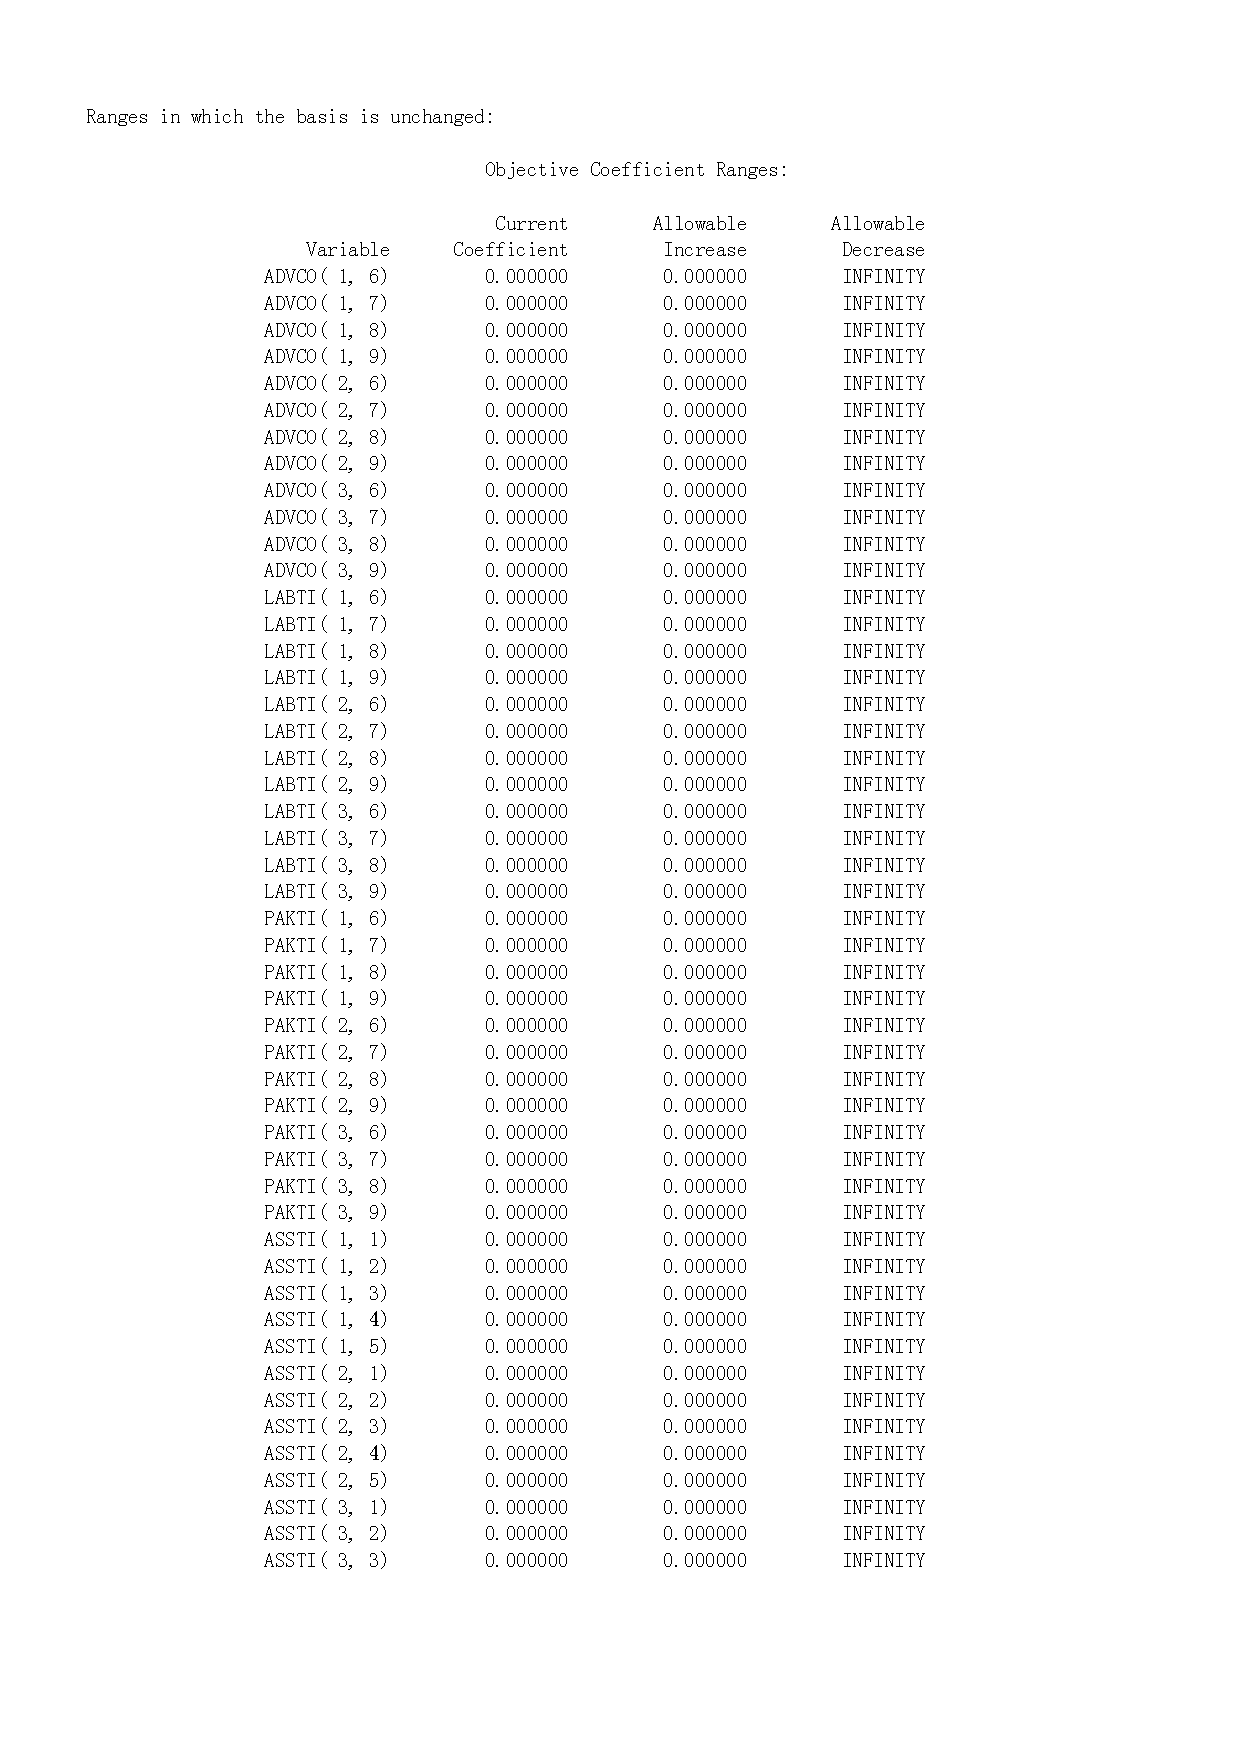
\includepdf[pages={1,2,3,4,5,6}]{solution_reprot.pdf}

\end{document}